
\documentclass{standalone}

\usepackage{amsmath} 
\usepackage{tikz}

\begin{document}
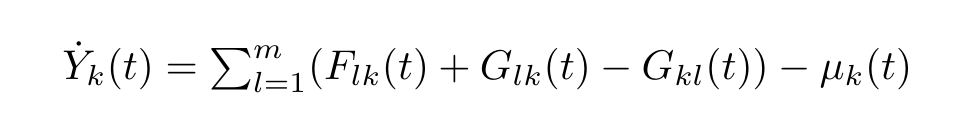
\begin{tikzpicture}
\node[scale=1.5] {
$
\begin{array}{l}
%k \in \{ 1,\ldots,m \} : \\
%
\dot{Y}_k(t) = \sum_{l=1}^{m} ( F_{lk}(t) + G_{lk}(t) - G_{kl}(t) ) - \mu_{k}(t) 
\end{array}
$
};
\end{tikzpicture}
\end{document}

